% =====================================================================
% FINESST-25 (NNH25ZDA001N) — ANONYMIZED TECHNICAL PROPOSAL — FULL DRAFT
% File 1 of 2: S/T/M (max 6 pp) + References + OSDMP (max 2 pp)
%              + Mentoring Plan (max 2 pp)
%
% DAPR: no names/institutions outside the reference list; numeric
% citations; no gendered pronouns; unsigned mentoring plan; scrub PDF
% metadata (keep \hypersetup pdfauthor EMPTY). Full author names ARE
% allowed inside the reference list.
%
% STATUS: complete draft. Red \todo{} items = facts to verify or
% numbers to fill. Two figure slots reserved; after inserting figures,
% check the 6-page S/T/M limit and trim §2 first if over.
% =====================================================================
\documentclass[12pt,letterpaper]{article}
\usepackage[margin=1in]{geometry}
\usepackage{newtxtext,newtxmath}
\usepackage{graphicx}
\usepackage{booktabs}
\usepackage{xcolor}
\usepackage[colorlinks=true,citecolor=blue,urlcolor=blue,linkcolor=blue,
            pdftitle={FINESST Proposal},pdfauthor={}]{hyperref}
\usepackage{titlesec}
\titlespacing*{\section}{0pt}{7pt}{3pt}
\titlespacing*{\subsection}{0pt}{5pt}{2pt}
\titleformat*{\section}{\large\bfseries}
\titleformat*{\subsection}{\normalsize\bfseries}
\setlength{\parskip}{2pt}
\pagestyle{plain}

\newcommand{\todo}[1]{\textcolor{red}{[TODO: #1]}}
\newcommand{\lya}{Ly$\alpha$}
\newcommand{\xhi}{x_{\rm HI}}

\begin{document}

% =====================================================================
% S/T/M — MAX 6 PAGES
% =====================================================================
\begin{center}
{\large\bfseries Mapping Reionization-Era Ionized Bubbles by Recovering
Lyman-$\alpha$ Information from Low-Resolution JWST and Roman
Spectroscopy}\\[2pt]
{\itshape Science/Technical/Management Section}
\end{center}

\section{Science Goals and Objectives}
\label{sec:goals}

The Epoch of Reionization (EoR) --- the last major phase transition of
the Universe, during which the first luminous sources ionized the neutral
intergalactic medium (IGM) --- remains one of the frontier problems of
galaxy formation and cosmology [1,2]. While the broad timing of
reionization is now bracketed ($z\sim5.5$--$10$; [3,4]), its
\emph{morphology} is not: we do not yet know the characteristic sizes of
ionized bubbles at a given epoch, how they grew and merged, or which
galaxy populations drove that growth. The ionized bubble size
distribution (BSD) as a function of redshift is the key observable that
discriminates between reionization scenarios --- early versus late,
gradual versus rapid, and driven by faint numerous galaxies versus rare
luminous systems [5,6,7].

The \lya\ emission line of $z\gtrsim7$ galaxies is the most direct
available probe of this morphology. A \lya\ photon escaping a galaxy
embedded in a small ionized bubble encounters nearby neutral hydrogen and
is strongly attenuated by the damping wing; a photon emitted inside a
large bubble redshifts safely out of resonance before reaching the
neutral IGM and survives [8,9]. Consequently the visibility, equivalent
width, and velocity profile of \lya\ encode the size of the local ionized
region [10,11]. JWST has transformed this field by detecting \lya\ from
galaxies deep into the EoR, including surprisingly strong emitters at
$z=7$--$11$ interpreted as sitting inside early large bubbles [12,13,14].
Yet current constraints rest on small samples of individually modeled
objects. Measuring the BSD --- a population-level statistic --- requires
extracting IGM transmission information from \emph{hundreds} of spectra,
and there lies the obstacle: statistically large EoR samples exist almost
exclusively at low spectral resolution, where the diagnostic information
in the line is smeared away. The JWST/NIRSpec prism ($R\sim30$--$300$)
dominates existing $z>7$ spectroscopy, and the Roman Space Telescope
grism ($R=461\lambda/\mu$m over 1--1.93~$\mu$m) will soon deliver the
widest-area EoR spectroscopy ever taken --- both at resolutions where
\lya\ velocity structure is unresolved.

This proposal will break that resolution barrier with a validated,
physics-informed deep-learning framework, and use it to deliver the first
statistical measurement of the ionized bubble size distribution at
$z=7$--$9$ from \lya\ observables. Recent work [15] demonstrated a
physics-informed super-resolution (SR) framework that enhances real
JWST/NIRSpec prism spectra by a factor of $\sim$10 in resolving power
($R\sim100\rightarrow R\sim1000$), trained on $\sim$1,200 paired
prism--grating observations from the public JADES survey; the framework
deblends closely spaced emission features (e.g., the
[O\,\textsc{iii}]$\lambda\lambda$4959,5007 doublet and H$\beta$),
improves emission-line S/N by factors of several, and returns calibrated,
wavelength-dependent uncertainties. The proposed research builds on this
foundation through three objectives:

\begin{itemize}\setlength\itemsep{1pt}
\item \textbf{Objective 1 --- Validate \lya\ information recovery from
low-resolution spectra.} Quantify, using held-out JADES prism--grating
pairs and simulation-based falsification tests, which \lya\ diagnostics
(equivalent width, line centroid relative to systemic redshift, and
damping-wing continuum shape) are recoverable from prism data, and
compare super-resolve-then-infer against direct low-resolution inference
(\S\ref{sec:task1}).
\item \textbf{Objective 2 --- Measure the bubble size distribution at
$z=7$--$9$.} Couple the validated spectral inference to a neural
posterior model trained on radiative-transfer (RT) simulations of the
reionizing IGM, apply it to the public JADES $z=7$--$9$ prism sample
($>$100 galaxies), and infer the population-level BSD with a hierarchical
framework that uses detections, non-detections, and upper limits
(\S\ref{sec:task2}).
\item \textbf{Objective 3 --- Make the measurement Roman-ready.} Adapt
the framework to Roman grism spectroscopy, where \lya\ enters the
bandpass at $z\gtrsim7.2$, using public Roman grism simulation products
and an already-working end-to-end extraction pipeline, so that the BSD
measurement can be extended to the rare, luminous galaxies tracing the
largest bubbles as soon as Roman survey data become public
(\S\ref{sec:task3}).
\end{itemize}

If successful, this program will convert the largest existing and
forthcoming EoR spectroscopic samples --- currently used mainly for
redshift confirmation --- into a quantitative map of reionization's
morphology, providing a direct observational test of whether ionized
bubbles at $z\sim8$ follow the size distributions predicted by
galaxy-driven reionization models [5,6] or require rarer, more luminous
drivers [14,16]. All data used are from NASA missions: public JWST
archival spectroscopy and Roman preparation products.

\section{Scientific Background}
\label{sec:background}

\subsection{Ionized bubbles and \lya\ observables}
During reionization, ionized regions grow around biased sources,
percolate, and merge; analytic models and simulations predict a
characteristic bubble scale growing from $\lesssim$1 comoving Mpc when
the IGM is mostly neutral to tens of cMpc as reionization completes
[5,6,7]. For a galaxy at systemic redshift $z_{\rm sys}$ inside a bubble
of proper radius $R_b$, the \lya\ damping-wing optical depth at line
center scales inversely with the distance the photon travels before
encountering neutral gas; transmission rises steeply with $R_b$ up to
$\sim$1~pMpc [8,10]. Three observables carry this signal at low
resolution: (i) the \lya\ \emph{equivalent width} distribution, whose
evolution at $z>6$ is the classic neutral-fraction probe [11,17]; (ii)
the \emph{velocity offset} of the transmitted line peak from systemic ---
larger offsets survive smaller bubbles, so the offset distribution maps
bubble sizes when systemic redshifts are known from other lines
[10,18]; and (iii) the \emph{damping-wing imprint} on the continuum
redward of the break [9,19]. JWST spectroscopy has produced both striking
individual cases --- strong \lya\ at $z=8$--$11$ implying early
$\gtrsim$1--3~pMpc bubbles [12,13,14] --- and growing statistical samples
[20,21]. What is missing is a method that extracts profile-level
information from the low-resolution spectra that constitute the bulk of
the data, and a forward-modeling framework that turns a heterogeneous
population of detections and limits into a BSD measurement. That is
precisely what this proposal provides.

\subsection{The low-resolution bottleneck and validated super-resolution}
At the NIRSpec prism resolution near 1~$\mu$m ($R\sim50$), one resolution
element spans several thousand km\,s$^{-1}$: \lya\ velocity offsets
(typically 100--500 km\,s$^{-1}$) and line asymmetries are unresolved,
and the line blends into the continuum break. Medium-resolution gratings
resolve these diagnostics but exist for only a small fraction of EoR
targets. The SR framework of [15] was built to bridge exactly this gap:
a three-stage architecture (a conservative convolutional SR stage with
per-pixel uncertainty; a redshift-inference head; and a physics-informed
refinement stage in which $\sim$80 known emission features are modeled as
attention-gated parametric line profiles added to a smooth continuum
correction) trained end-to-end on \emph{real} paired prism/grating
JADES observations rather than idealized simulations. On held-out test
data the framework achieves noise-limited residuals over most of the
spectral range and recovers redshift information approaching that of the
high-resolution reference spectra [15].

Two properties make this framework suitable for trustworthy \emph{science}
--- not just visually sharper spectra. First, it produces calibrated
wavelength-dependent uncertainties, enabling propagation into downstream
inference. Second, and critically, an accompanying falsification
methodology (a ``prior-dominance'' audit) measures whether the model
reads the data or recites its training prior: known perturbations are
injected into the underlying high-resolution truth, forward-modeled into
the low-resolution input, and the recovered response is measured as an
exponent $r$ ($r=1$: fully data-driven; $r=0$: pure prior). This audit,
developed in the Roman-adaptation work described in \S\ref{sec:task3},
exposed prior-dominated behavior in an unaugmented model ($r\simeq0.35$)
and directly motivated the physics-based augmentation strategy that
mitigates it. This built-in capacity for self-falsification addresses the
central and legitimate skepticism about ML-reconstructed spectra, and is
carried through every task below.

% ---------------- FIGURE 1 ----------------
\begin{figure}[t]
\centering
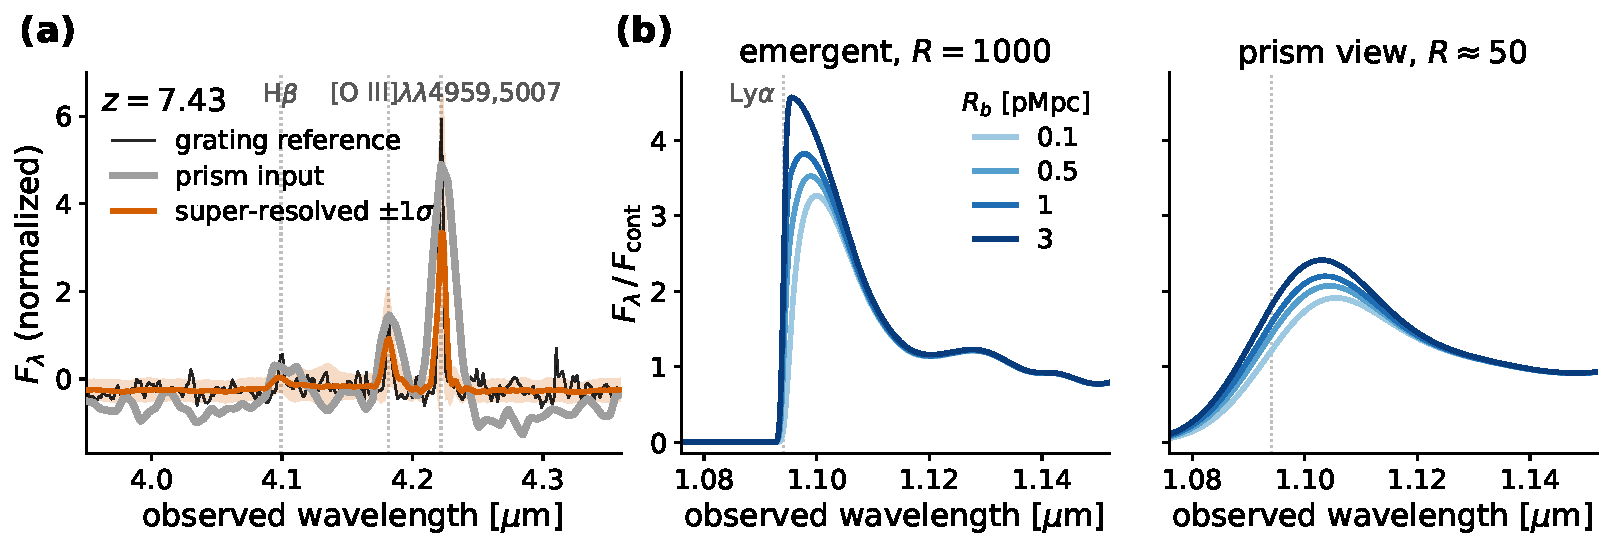
\includegraphics[width=\textwidth]{figure1.pdf}
\caption{\small \textbf{(a)} A JADES galaxy at $z=7.43$: the NIRSpec
prism spectrum (grey), the medium-resolution grating reference (black),
and the super-resolved output of the framework [15] with $1\sigma$
uncertainty (color). The prism blends H$\beta$ and the [O\,III] doublet
into a single broad feature; the super-resolved spectrum recovers all
three lines at grating resolution. \textbf{(b)} A fixed intrinsic \lya\
profile (median of JADES $z\simeq4$--$5.5$ \lya-emitter templates)
transmitted through ionized bubbles of $R_b=0.1$--$3$ pMpc at $z=8$
(Miralda-Escud\'e damping wing, $\bar{x}_{\rm HI}=0.5$ outside the
bubble), shown at $R=1000$ (left) and convolved to prism resolution
(right): the bubble-size signature that is unresolved in the prism data
is the information this program recovers and exploits.}
\label{fig:one}
\end{figure}

\section{Technical Approach and Methodology}
\label{sec:approach}

\subsection{Task 1: Validated \lya\ recovery from prism spectra (Year 1)}
\label{sec:task1}
\textbf{T1.1 --- \lya\ training and validation set.} From the 1,187
paired prism--grating observations already assembled from the public
JADES data releases [22], the subset with coverage of \lya\ at $z>5.5$
will be identified with the existing ingestion pipeline. Because the IGM is largely transparent at
$z\simeq4$--$5.5$, several hundred additional JADES spectra at those
redshifts provide intrinsic-profile templates; a mock-generation pipeline
(already prototyped) multiplies these templates by simulated IGM
transmission curves and convolves to prism resolution, yielding a
controlled test bed where the true transmission is known.

\textbf{T1.2 --- Fine-tune and audit the SR framework on the \lya\
region.} The pretrained framework of [15] will be fine-tuned with a
loss emphasizing the \lya\ line and adjacent continuum, including the
resonant-line asymmetry. The prior-dominance audit will be extended to
\lya: transmission curves perturbed off the training manifold
(systematically larger/smaller bubbles, damping-wing shapes from
different $\xhi$) are forward-modeled to prism resolution and the
response exponent $r$ measured per diagnostic. Acceptance criterion:
$r\gtrsim0.7$ for equivalent width and centroid; diagnostics failing the
audit are excluded from downstream inference rather than patched.

\textbf{T1.3 --- The decisive comparison: SR-then-infer vs.\ direct
inference.} Information not present in the prism data cannot be created
by SR; its value must be demonstrated, not assumed. On identical mocks,
two chains will be compared end-to-end: (a) direct neural inference of
transmission parameters from the prism spectrum, and (b) inference from
the super-resolved spectrum with propagated uncertainties. The comparison
--- per-diagnostic bias, scatter, and calibration --- fixes the
architecture for Task 2 and is itself a publishable methods result
(planned publication~1). Either outcome advances the science: if SR adds
recoverable information (as the deblending results of [15] indicate),
the gain is quantified; if not, the direct chain proceeds with the same
validation machinery. \emph{This task therefore cannot fail its own
premise.}

\subsection{Task 2: The bubble size distribution at $z=7$--$9$ (Years 1--2)}
\label{sec:task2}
\textbf{T2.1 --- Simulation training set.} Per-sightline \lya\
transmission curves with known local bubble sizes will be drawn from RT
simulations of patchy reionization spanning $z\simeq6$--$9$ and a range
of global neutral fractions. Three sources ensure robustness against
simulation choice: (i) a suite of RT post-processed hydrodynamic
simulations already in hand (obtained via private consultation),
providing $10^4$ sightlines per snapshot with matched ionization cubes
from which multi-ray mean-free-path bubble labels are computed (pipeline
already built and tested); (ii) the public THESAN \lya\ transmission
catalogs [23]; and (iii) the public SPHINX$_{20}$ data release [24].
Cross-simulation training/testing quantifies model dependence of the
labels --- reported as a systematic error component, not hidden.

\textbf{T2.2 --- Per-galaxy posterior inference.} A neural posterior
estimator (simulation-based inference; [25]) will map the recovered
\lya\ observables --- with their calibrated uncertainties --- to a
posterior over local bubble size $R_b$ and line-of-sight transmission,
conditioned on galaxy properties (UV magnitude, systemic redshift
quality). Mock-recovery experiments establish coverage (posterior
calibration) before any application to data.

\textbf{T2.3 --- Population-level BSD.} A hierarchical Bayesian layer
combines per-galaxy posteriors --- including non-detections and upper
limits, which carry much of the information at $z>7$ --- into the BSD at
$z\simeq7$, 8, and 9, marginalizing over intrinsic EW distribution
parameters [11]. The result will be confronted with predictions of
galaxy-driven semi-numeric models [6,7] and the RT suites of T2.1.

\textbf{T2.4 --- Application sample.} The primary sample is the public
JADES prism sample: 108 galaxies at $z=7$--$8$ are already extracted
with the existing pipeline, to be extended to $z=8$--$9$ from the same
public releases and supplemented by other public NIRSpec programs whose
prism spectra cover \lya\ at $z>7$ --- CEERS, UNCOVER, and RUBIES, all
with team-released reduced spectra (via MAST and the DAWN JWST
Archive). Systemic redshifts come from strong rest-optical lines in the
same spectra ([O\,\textsc{iii}], H$\beta$), for which the SR framework
was originally validated [15]. Planned publication~2 (flagship): the
first statistical BSD at $z=7$--$9$ from \lya\ observables.

\subsection{Task 3: Extension to Roman grism spectroscopy (Years 2--3)}
\label{sec:task3}
Roman's wide-area grism spectroscopy will observe of order a thousand
square degrees at $R=461\lambda/\mu$m over 1--1.93~$\mu$m [26,27]; \lya\
enters this bandpass at $z\gtrsim7.2$. Roman will thus capture the
bright ($M_{\rm UV}\lesssim-22$), rare galaxies that JWST's deep pencil
beams miss --- exactly the population expected to trace the largest
ionized bubbles [14,16] --- over volumes two orders of magnitude beyond
existing surveys.

\textbf{T3.1 --- Simulation-based grism pipeline (complete/in hand).} An
end-to-end pipeline operating on the public Roman grism simulation
products [28] (hosted at IRSA) has already been developed as
groundwork: it prepares the simulated 2D slitless frames, builds
full-field contamination models, performs optimal 1D extraction with a
wavelength solution validated to sub-pixel accuracy (median error
$-3$~\AA\ on emission-line knots), and has produced $>$17,000
low-/high-resolution training pairs, with $\sim$250,000 expected from the
full 15-field products. The SR stage retrained on these data recovers
emission lines at 80--95\% of true amplitude for line S/N $\gtrsim5$.

\textbf{T3.2 --- High-$z$ injection and \lya\ recovery.} The public
simulation products contain $0<z<3$ galaxies only; EoR sources will
therefore be \emph{injected}: mock \lya\ lines and damping-wing continua
from T2.1, plus realistic interlopers, dispersed into the 2D frames
through the validated pipeline, then recovered end-to-end. This yields
Roman-specific completeness, purity, and $R_b$-recovery functions versus
magnitude and line flux --- the quantitative forecast for Roman's EoR
bubble census (planned publication~3).

\textbf{T3.3 --- Deployment path and data risk statement.} This project
does \emph{not} depend on unreleased data: Objectives~1--2 use public
JWST archives, and Objective~3's deliverables are validated on public
simulation products. Real Roman wide-area spectroscopy, expected within
the award period following launch ($\sim$2027), will be used as an
opportunity as soon as it is public: the T3.2 machinery applies without
modification, and cross-instrument overlap samples will anchor
sim-to-real domain adaptation. If Roman data are delayed beyond the award
period, the contingency is expansion of Task~2 to the full public JWST
archive; Objectives~1--2 and all three publications remain achievable.

\subsection{Anticipated setbacks and mitigation}
\begin{itemize}\setlength\itemsep{0pt}
\item \emph{SR adds little for \lya\ specifically} $\rightarrow$ T1.3 is
designed as a decision experiment; the direct-inference chain uses the
same validation machinery (methods paper either way).
\item \emph{Simulation dependence of bubble labels} $\rightarrow$
three independent simulation suites (T2.1); cross-training systematic
budget; prior-dominance audit per diagnostic.
\item \emph{Small \lya-emitter samples at $z>8$} $\rightarrow$ the
hierarchical BSD framework (T2.3) is built for censored data;
non-detections constrain the small-bubble end.
\item \emph{Roman schedule slip} $\rightarrow$ explicit JWST-only
contingency (T3.3).
\end{itemize}

\subsection{Computing resources}
Model training is modest by ML standards ($\sim$2.5M-parameter networks;
datasets $\lesssim$10~GB): all tasks are executable on a dedicated
research-group GPU system (NVIDIA RTX 5090 class) supplemented by the
institutional GPU cluster, both described in the Expertise \& Resources
document. No NASA High-End Computing request is included.

\section{Relevance to NASA and the Astrophysics Division}
This investigation directly addresses the Astrophysics Division goals to
``probe the origin and destiny of our universe'' and ``explore the origin
and evolution of the galaxies,'' and is relevant to the Astrophysics
Research program. It is built exclusively on NASA
mission data and preparation products: public JWST/NIRSpec archival
spectroscopy from MAST (Objectives 1--2) and Roman grism simulation
products from IRSA in direct preparation for Roman's core community
surveys (Objective 3). Beyond the specific EoR science, the validated
spectral-inference methodology --- with built-in falsification audits and
calibrated uncertainties --- is directly transferable to Roman's
survey-scale emission-line science and to spectroscopy with future
missions such as the Habitable Worlds Observatory. All software, trained
models, and catalogs will be publicly released (see OSDMP).

\section{Work Plan, Schedule, and Milestones}
\label{sec:schedule}
\begin{center}\small
\begin{tabular}{p{0.65in}p{4.6in}}
\toprule
\textbf{Year 1} & T1.1--T1.3 complete; \lya\ audit results; SR-vs-direct
decision; T2.1 multi-simulation training set assembled. \emph{Milestone:}
methods paper submitted (publication 1). Conference presentation (AAS). \\
\textbf{Year 2} & T2.2--T2.4: posterior calibration, hierarchical BSD from
JADES + public archive at $z=7$--9. \emph{Milestone:} flagship BSD paper
submitted (publication 2). T3.2 injection framework running. \\
\textbf{Year 3} & T3.2--T3.3: Roman forecast paper (publication 3);
application to early public Roman data if available; public release of
code, trained models, and catalogs; thesis completion. \\
\bottomrule
\end{tabular}
\end{center}

\noindent\textbf{Table of Personnel and Work Effort} (anonymized; the
identical table with names appears in the Expertise \& Resources
document):
\begin{center}\small
\begin{tabular}{lll}
\toprule
Role & Contribution & Effort \\
\midrule
FI & All analysis, pipeline development, publications & 1.0 FTE \\
PI & Thesis supervision, survey/spectroscopy guidance & no cost requested \\
Mentor 1 & ML methodology and spectroscopy co-mentoring & no cost requested \\
\bottomrule
\end{tabular}
\end{center}

% =====================================================================
% REFERENCES — numeric, full names allowed, not in page limit
% All entries verified against Crossref/publisher records 2026-07-09.
% =====================================================================
\clearpage
\begin{center}{\large\bfseries References}\end{center}
\begin{enumerate}\setlength\itemsep{0pt}\small
\item Robertson, B. E. 2022, ARA\&A, 60, 121
\item Loeb, A., \& Barkana, R. 2001, ARA\&A, 39, 19
\item Fan, X., et al. 2006, AJ, 132, 117
\item Planck Collaboration 2020, A\&A, 641, A6
\item Furlanetto, S. R., Zaldarriaga, M., \& Hernquist, L. 2004, ApJ, 613, 1
\item Mesinger, A., \& Furlanetto, S. 2007, ApJ, 669, 663
\item Lin, Y., et al. 2016, MNRAS, 461, 3361 % bubble size distributions
\item Miralda-Escud\'e, J. 1998, ApJ, 501, 15
\item Mortlock, D. J., et al. 2011, Nature, 474, 616 % z=7.085 quasar damping wing
\item Mason, C. A., et al. 2018, ApJ, 856, 2 % neutral fraction from Lya EW
\item Mason, C. A., et al. 2018, ApJ, 857, L11 % boosted Lya from UV-bright galaxies
\item Bunker, A. J., et al. 2023, A\&A, 677, A88 % GN-z11 Lya
\item Witstok, J., et al. 2024, A\&A, 682, A40 % JADES/FRESCO LAE environments
\item Tang, M., Stark, D. P., Chen, Z., et al. 2023, MNRAS, 526, 1657 % CEERS bright LAEs in ionized bubbles
\item Haghjoo, A., Hemmati, S., Mobasher, B., et al. 2026, arXiv:2603.18357 (submitted to ApJ)
\item Naidu, R. P., Tacchella, S., Mason, C. A., et al. 2020, ApJ, 892, 109 % oligarch reionization
\item Stark, D. P., et al. 2010, MNRAS, 408, 1628 % Lya fraction
\item Lu, T.-Y., Mason, C. A., Mesinger, A., et al. 2025, A\&A, 697, A69 % bubble mapping from Lya velocity offsets
\item Umeda, H., et al. 2024, ApJ, 971, 124 % damping-wing neutral fractions and bubble sizes at z=7-12
\item Saxena, A., et al. 2024, A\&A, 684, A84 % JADES faint LAEs
\item Jones, G. C., et al. 2025, MNRAS, 536, 2355 % JADES Lya reionization statistics
\item Curtis-Lake, E., et al. 2025, arXiv:2510.01033 % JADES DR4 Paper I
\item Smith, A., et al. 2022, MNRAS, 512, 3243 % THESAN Lya
\item Rosdahl, J., et al. 2022, MNRAS, 515, 2386 % SPHINX LyC escape
\item Cranmer, K., Brehmer, J., \& Louppe, G. 2020, PNAS, 117, 30055
\item Spergel, D., et al. 2015, arXiv:1503.03757 % Roman/WFIRST
\item Wang, Y., et al. 2022, ApJ, 928, 1 % Roman HLSS reference survey
\item Wang, Y., et al. 2022, Roman HLSS Grism Simulation Products, IRSA, doi:10.26131/IRSA548 % dataset accompanying [27]
\end{enumerate}

% =====================================================================
% OSDMP — MAX 2 PAGES, ANONYMIZED
% =====================================================================
\clearpage
\begin{center}{\large\bfseries Open Science and Data Management Plan}\end{center}

\noindent\textbf{(a) Data types, volumes, formats, and standards.}
This project uses only publicly available input data: JWST/NIRSpec
spectra from public JADES data releases and other public programs,
retrieved from MAST; and public Roman grism simulation products hosted at
IRSA. Radiative-transfer simulation sightlines are obtained from the
public THESAN and SPHINX releases and from a simulation suite available
to the team (obtained via private consultation); only derived,
shareable products of the latter (transmission curves and bubble-size
labels used for training) will be redistributed, with permission.
Generated products comprise: (i) curated training datasets
(HDF5/npz; $\lesssim$10~GB total); (ii) trained model weights with
configuration files ($<$1~GB); (iii) per-galaxy value-added catalogs
(\lya\ diagnostics, posteriors over bubble size; FITS and ECSV following
IVOA-compliant column metadata; $<$1~GB); and (iv) all analysis software
(Python). Formats follow community standards (FITS, HDF5, ECSV; PyTorch
checkpoint format for weights).

\noindent\textbf{(b) Repositories.}
Software will be developed openly in a public git repository from day
one and archived at Zenodo (with DOI) at each release. Trained models and
training datasets will be deposited on Zenodo and mirrored on a public
model hub. Value-added catalogs will be published as machine-readable
supplements to the associated journal articles, deposited on Zenodo, and
contributed to MAST as a High-Level Science Product if accepted. Interim
storage uses the research group's dedicated GPU server, which is
sufficient for the training sets and model checkpoints involved;
multi-TB project storage on the institutional high-performance
computing center is available should additional capacity be required.

\noindent\textbf{(c) Release timeline.}
Each dataset, model, and catalog is released no later than publication of
its associated paper (planned: methods, Year 1; BSD, Year 2; Roman
forecast, Year 3). As-accepted manuscripts are posted to arXiv at
acceptance. Any scientifically useful product not covered by a
publication is released by the end of the award.

\noindent\textbf{(d) Archiving responsibility and experience.}
The FI performs all curation and archiving, and has prior experience
releasing research software, trained checkpoints with model cards, and
documented pipelines through public repositories and model hubs (phrased
here without identifying links; see the Expertise \& Resources document).
The PI's group maintains long-term stewardship of the group's public data
products.

\noindent\textbf{(e) Software development and release.}
Software is developed under version control with continuous-integration
tests and documentation, released under a permissive open-source license
(BSD-3/MIT), with pinned environments (lock files) and end-to-end
examples sufficient to reproduce every figure and catalog in the
publications. Persistent identifiers: all team members maintain ORCIDs
linked in NSPIRES; datasets and software carry Zenodo DOIs cited in the
papers.

% =====================================================================
% MENTORING PLAN — MAX 2 PAGES, ANONYMIZED, UNSIGNED
% =====================================================================
\clearpage
\begin{center}{\large\bfseries Mentoring Plan}\end{center}

\noindent This plan was prepared jointly by the FI, the PI, and one
co-mentor (Mentor 1: machine-learning methodology and space-based
spectroscopy). It complements the research plan by defining how the FI
acquires the scientific breadth, technical depth, and professional
skills to complete the proposed program and transition to an independent
research career.

\noindent\textbf{1. Mentoring structure and cadence.}
The FI meets the PI weekly (research direction, progress against
milestones) and Mentor 1 weekly by video, supplemented by in-person
working sessions at Mentor 1's institution approximately every two
weeks (model design, validation methodology, survey spectroscopy). Guidance on IGM physics and the reionization
simulations is available through established expertise at the FI's
institution, including on the FI's thesis committee. A joint
all-mentors meeting is held quarterly to review milestones from the Work
Plan (\S6 of the S/T/M) and adjust scope; written quarterly goals are
agreed and revisited. The FI's institutional thesis committee provides an
independent annual assessment.

\noindent\textbf{2. Scientific and technical development.}
\emph{Year 1:} depth in reionization theory and \lya\ radiative transfer
(directed reading guided by the PI and institutional experts; graduate
IGM coursework as needed); statistical inference (simulation-based
inference, hierarchical modeling); completion of the
validation-methodology skill set with Mentor 1. \emph{Year 2:} population-level statistical analysis;
scientific writing leadership on the flagship paper; peer-review
apprenticeship (co-refereeing with the PI where journals permit).
\emph{Year 3:} survey-scale data engineering for Roman-ready deployment;
supervision experience by co-mentoring a junior student on a bounded
sub-project; thesis completion.

\noindent\textbf{3. Professional development and community integration.}
The FI presents annually at a major national meeting (e.g., AAS) and at
one topical workshop per year (EoR/\lya\ or astro-ML), with mentors
coaching talk preparation. The FI's regular in-person working sessions
at Mentor 1's institution (approximately biweekly; \S1) embed the FI in
that institution's survey-science community and build collaboration
networks beyond the immediate mentoring team. The FI participates in the relevant Roman
science community activities to prepare for survey data, and in journal
clubs and group meetings across the mentoring team. Travel costs are
budgeted in the E\&R document.

\noindent\textbf{4. Career planning.}
Semi-annual career conversations with the PI cover trajectory,
fellowship and postdoctoral applications (application cycle prepared in
Year 3 with mentor review of materials), and building a recognizable
independent research identity at the intersection of EoR science and
trustworthy ML. The mentoring team commits to timely recommendation
letters and to nominating the FI for early-career opportunities
(conference talks, science-team memberships).

\noindent\textbf{5. Assessment.}
Progress is assessed against the milestone table in the S/T/M: submission
of publications 1--3, public releases of code/models/catalogs, and
conference presentations. If a milestone slips by more than one quarter,
the mentoring team and FI jointly re-scope using the mitigation options
identified in the research plan (\S3.4 of the S/T/M). The plan itself is
revisited annually and updated by mutual agreement.

\noindent\emph{(This plan is intentionally unsigned in accordance with
dual-anonymous review requirements.)}

\end{document}
